\documentclass[12pt,aspectratio=169]{beamer}
\usetheme{aurigapolimi}

\setbeamertemplate{bibliography item}{\insertbiblabel}

% % % % METADATA % % % % % % % % % % % % 

\title{Clustering of Spatial Data}
\subtitle{An application to early childhood education and care
services and their impact on women’s labour market}
\author{
  Tommaso Baresi, 
  Luca Perego, 
  Paul Poupeau, \\
  Leonardo Tisato,
  Alexis Toppé,
  Anh Chi Tuan} 

\institute{February 19\textsuperscript{\tiny{th}}, 2026 }
\setaurigadate{}
\selectcolor{deepBluePolimi} % lighter polimi blue also available (bluePolimi)


% = = = = = = = = = = = = = = = = = = = =
% Set up logos = = = = = = = = = = = = =
% = = = = = = = = = = = = = = = = = = = =

% Title-page logos
\setaurigatitlelogoA{logos/polimi_logo.eps}
\setaurigatitlelogoheightA{1.5cm}

%\setaurigatitlelogoB{logos/uab_text.eps}
%\setaurigatitlelogoheightB{1.8cm}

% Slide logos
\setaurigalogoA{logos/polimi_logo.eps}
\setaurigalogoheightA{0.5cm}

%\setaurigalogoB{logos/}
\setaurigalogoheightB{}

\begin{document}
\aurigatitleframe

\newcommand{\iid}{\stackrel{\tiny{iid}}{\sim}}
\newcommand{\ind}{\stackrel{\tiny{ind}}{\sim}}

\include{slides_second_presentation/0_Introduction}

\section{Dataset Overview}

\begin{frame}{Dataset Overview}

\begin{columns}[T]

    \column{0.5\textwidth}
    \vspace{0.5 cm}
    \textbf{Analysis of a geojson file}
    \begin{itemize}
    \item Data from 2022 \\
    \item Main source: ISTAT
    \item 107 provinces
    \item 47 numerical variables \\
    16 \underline{non} numerical variables
    \item \underline{No} missing values
    \end{itemize}
    
    \column{0.43\textwidth}
    \centering
    
\includegraphics[width=0.8\linewidth]{pictures/provinces_map.png}

\end{columns}

\end{frame}


\section{Exploratory Data Analysis} 

\begin{frame}{Spatial Visualization}

    \vfill
    
    \begin{center}
        Female employment rate and ECEC coverage by province
        
        \vspace{0.3 cm}
        
        
\includegraphics[width=0.72\linewidth]{pictures_first_presentation/fem_emp_rate_and_ECEC_map.png}
    \end{center}
    
    \vfill
    
\end{frame}


\begin{frame}{Moran's I Cluster}

    \vfill

    \begin{center}
        Female employment rate and ECEC coverage cluster
        
        
\includegraphics[width=0.7\linewidth]{pictures_first_presentation/morans_clusters_inverted.png}
    \end{center}

    \vfill
    
\end{frame}

\section{Variable selection} 

\begin{frame}{Variable Selection}
Goal : identify the most relevant predictors.\\

\vspace{0.5cm}
1. Remove variables considered irrelevant by the sociological literature (ex : \texttt{urban\_type}, \texttt{area\_km2}, ...);\\
% 2. Drop the variables with a Pearson or Spearman’s correlation coefficient $|\rho_{ij} | \leq 0.85$ with women’s employment rate
\vspace{0.5cm}
2. Remove variables highly correlated with the female employment rate ($|\rho | \geq 0.85$), as they partially convey the same information (ex : \texttt{empl\_rate}, \texttt{unempl\_rate}, \texttt{fem\_house\_rate}, ...)


\end{frame}


\begin{frame}{Variable Selection}
3. Mitigate multicollinearity inside the ECEC group and Non-ECEC group\\
\vspace{0.5cm}
\begin{center}
    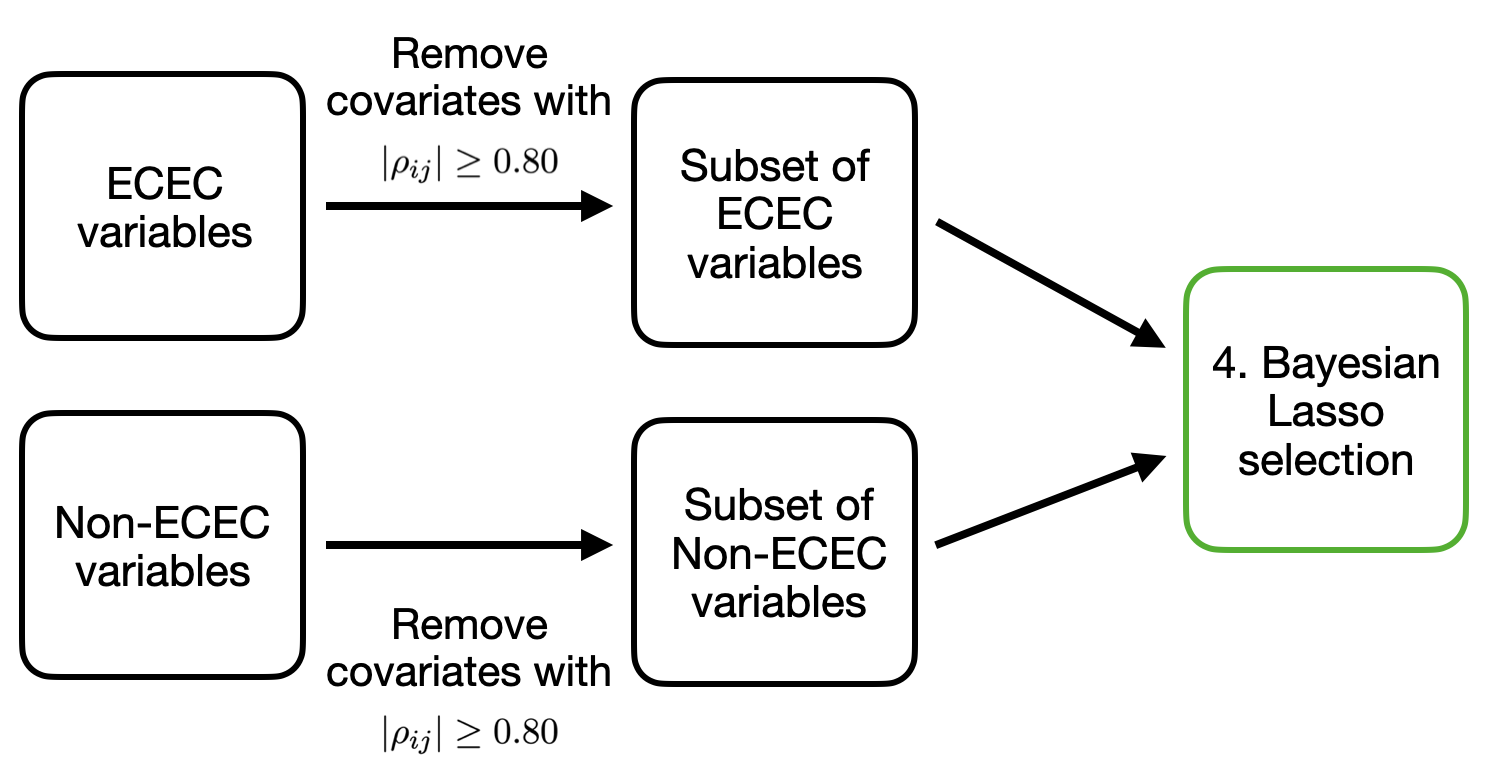
\includegraphics[scale=0.35]{pictures_second_presentation/illus_variable_selec.png}
\end{center}



\end{frame}




\begin{frame}{Bayesian Lasso}
\footnotesize
\begin{align*}
    y^{\ast}_i \mid \boldsymbol{\beta}, \sigma, \phi_i 
        &\stackrel{\text{ind}}{\sim}\mathcal{N}\big(\alpha + \phi_i +  \boldsymbol{x}_i^{\ast \top} \boldsymbol{\beta},\, \sigma^2\big) \, ,
        \quad i = 1,\dots,N \\
    \beta_j \mid \lambda, \sigma 
        &\stackrel{\text{iid}}{\sim}\mathrm{Laplace}\big(0,\, \sigma / \lambda\big) \, ,
        \quad j = 1,\dots,P \\
    \lambda^2 &\sim \mathrm{Gamma}(2, 1), \\
    \sigma &\sim \mathrm{HalfNormal}(1), \\
    \alpha &\sim \mathcal{N}\big(0, \, 10^2),\\
    \phi \mid \tau_c, \rho, W &\sim \mathcal{N}_N \big(\boldsymbol{0},[\tau_c (D -\rho W)]^{-1} \big),\\
    \rho &\sim \mathrm{Beta}(2,2),\\
    \tau_c &\sim \mathrm{Gamma}(1,1).\\
\end{align*}  

Selection criterion : 95\% credible interval does \underline{not} contain $0$

\end{frame}

\begin{frame}{Selection Results}
    \begin{center}
         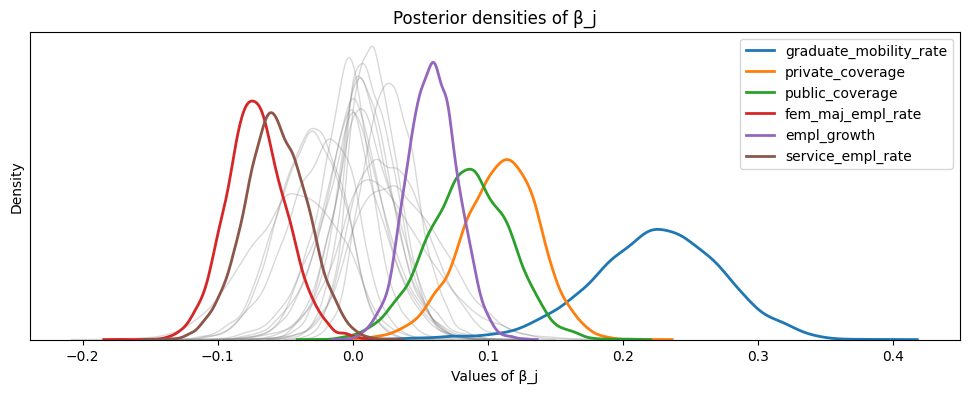
\includegraphics[scale=0.47]{pictures_second_presentation/final_variable_selection.png}
    \end{center}
         
         \footnotesize \textbf{Selected Variables} \scriptsize
         \begin{itemize}
             \item ECEC variables : \texttt{private\_coverage, public\_coverage}
             \item Non-ECEC variables : \texttt{fem\_maj\_empl\_rate, service\_empl\_rate,\\ graduate\_mobility\_rate, empl\_growth}
         \end{itemize}

\end{frame}




\begin{section}{Clustering}
\begin{frame}{Sparse Finite Mixture Model}
\tiny
\begin{align*}
y_i^\ast \mid \alpha,\boldsymbol{\pi},\{\boldsymbol{\beta}_k,\sigma_k^2\}_{k=1}^K,\phi_i
&\sim \sum_{k=1}^K \pi_k\,
\mathcal{N}\!\Big(\alpha+\mathbf{x}_i^{\ast\top}\boldsymbol{\beta}_k+\phi_i,\ \sigma_k^2\Big),
\qquad i=1,\dots,N\\
\boldsymbol{\pi} &\sim \mathrm{Dirichlet}\!\big(0.5\,\mathbf{1}_K\big),\\
\alpha &\sim \mathcal{N}(0,2),\\
\beta_{j,k}\mid b_{j,k},\lambda_{j}
&\stackrel{\text{ind}}{\sim} \mathcal{N}\!\Big(b_{j,k},\ \lambda_{j} \Big),
\qquad j=1,\dots,P,\ k=1,\dots,K\\
b_{j} &\stackrel{\text{iid}}{\sim} \mathcal{N}(0,1),
\qquad j=1,\dots,P\\
\lambda_{j} &\stackrel{\text{iid}}{\sim} \mathrm{Gamma}(0.5,0.5), \,
\qquad j=1,\dots,P\\
\sigma^2_k = \frac{1}{\nu_k}, \qquad \nu_k &\stackrel{\text{iid}}{\sim} \mathrm{Gamma}(2,1),
\qquad k=1,\dots,K\\
\phi_i &= \phi_{\mathrm{raw},i}-\frac1N\sum_{i'=1}^N \phi_{\mathrm{raw},i'},
\qquad i=1,\dots,N\\
\boldsymbol{\phi}_{\mathrm{raw}}\mid \tau,\rho,W
&\sim \mathcal{N}_N\!\Big(
\mathbf{0},\ \big[\tau\{\rho(D-W)+(1-\rho)I_N\}\big]^{-1}
\Big),\\
\tau &\sim \mathrm{Gamma}(2,1),\\
\rho &\sim \mathrm{Beta}(1,1).
\end{align*}

\end{frame}

\begin{frame}{Label Assignment}
\footnotesize
   \begin{itemize}
      \item \textbf{Latent labels:} for each province $i$, $z_i \in \{1,\dots,K\}$.
      \item \textbf{Component mean:} $\mu_{ik} = \alpha + {x_i^*}^\top \beta_k + \phi_i$.
      \item \textbf{Allocation weights:} $w_{ik} = \pi_k \, \mathcal{N}\!\left(y_i^* \mid \mu_{ik}, \sigma_k^2\right)$,\quad
            $r_{ik} = \dfrac{w_{ik}}{\sum_{h=1}^K w_{ih}}$.
      \item \textbf{Sampling step:} $z_i \mid r_i \sim \text{Categorical}(r_i)$ (one label vector per posterior draw).
      \item \textbf{Posterior Similarity Matrix (PSM):} $S_{ii'} = \Pr(z_i = z_{i'} \mid \text{data}) \approx \frac{1}{M}\sum_{m=1}^M \mathbb{I}\!\left(z_i^{(m)}=z_{i'}^{(m)}\right)$.
      \item \textbf{Point estimate of the partition (Binder loss):} choose $\hat z$ minimizing
            $\sum_{i<i'} \left[a\, S_{ii'}\,\mathbb{I}(\hat z_i \neq \hat z_{i'}) + b\, (1-S_{ii'})\,\mathbb{I}(\hat z_i = \hat z_{i'})\right]$.
      \item \textbf{Output:} $\hat z$ gives the final cluster labels used for interpretation.
    \end{itemize}
\end{frame}

\begin{frame}{Estimate cluster-specific coefficients}
\tiny
\begin{align*}
y_i^\ast \mid \alpha,\boldsymbol{\beta}_{c_i},\phi_i,\sigma_{c_i}
&\stackrel{\text{ind}}{\sim} \mathcal{N}\!\Big(\alpha+\mathbf{x}_i^{\ast\top}\boldsymbol{\beta}_{c_i}+\phi_i,\ \sigma_{c_i}^{2}\Big),
\qquad i=1,\dots,N\\
\alpha &\sim \mathcal{N}(0,2),\\
\beta_{j,c}\mid b_{j,c},\lambda_{j}
&\stackrel{\text{ind}}{\sim} \mathcal{N}\!\Big(b_{j,c},\ \lambda_{j} \Big),
\qquad j=1,\dots,P,\ c=1,\dots,C\\
b_{j,c} &\stackrel{\text{iid}}{\sim} \mathcal{N}(0,1),
\qquad j=1,\dots,P,\ c = 1,\dots,C\\
\lambda_{j} &\stackrel{\text{iid}}{\sim} \mathrm{Gamma}(0.5,0.5), \,
\qquad j=1,\dots,P\\
\sigma^2_c = \frac{1}{\nu_c}, \qquad \nu_c &\stackrel{\text{iid}}{\sim} \mathrm{Gamma}(2,1),
\qquad c=1,\dots,C\\
\phi_i &= \phi_{\mathrm{raw},i}-\frac1N\sum_{i'=1}^N \phi_{\mathrm{raw},i'} \, ,
\qquad i=1,\dots,N\\
\boldsymbol{\phi}_{\mathrm{raw}}\mid \tau,\rho,W
&\sim \mathcal{N}_N\!\Big(
\mathbf{0},\ \big[\tau\{\rho(D-W)+(1-\rho)I_N\}\big]^{-1}
\Big),\\
\tau &\sim \mathrm{Gamma}(2,1),\\
\rho &\sim \mathrm{Beta}(1,1).
\end{align*}
\end{frame}

\end{section}

\begin{frame}{Results}
\begin{itemize}
    \item 1 cluster recovered after the label assignment step.
    \item Posterior summaries for intercept and regression coefficients after fitting the model with $C=1$:
\end{itemize}
\normalsize
\begin{figure}
    \centering
    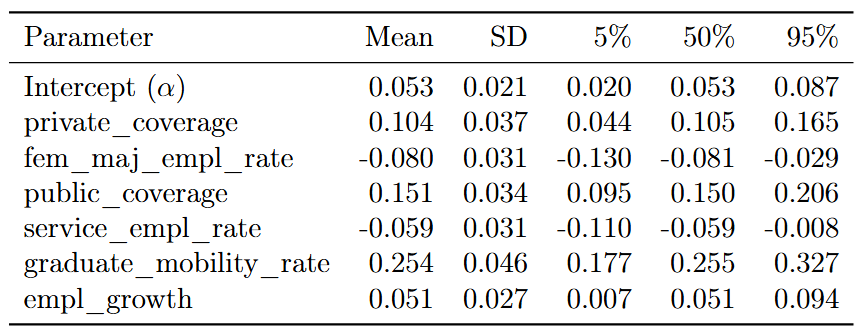
\includegraphics[width=0.7\linewidth]{slides_second_presentation/res.png}
    \caption{}
    \label{fig:res}
\end{figure}
\end{frame}


\begin{frame}{Results}
\begin{itemize}
    \item Posterior mean of the spatial random effects (left) and Observed female employment rate by province (right):
\end{itemize}
\begin{figure}
    \centering
    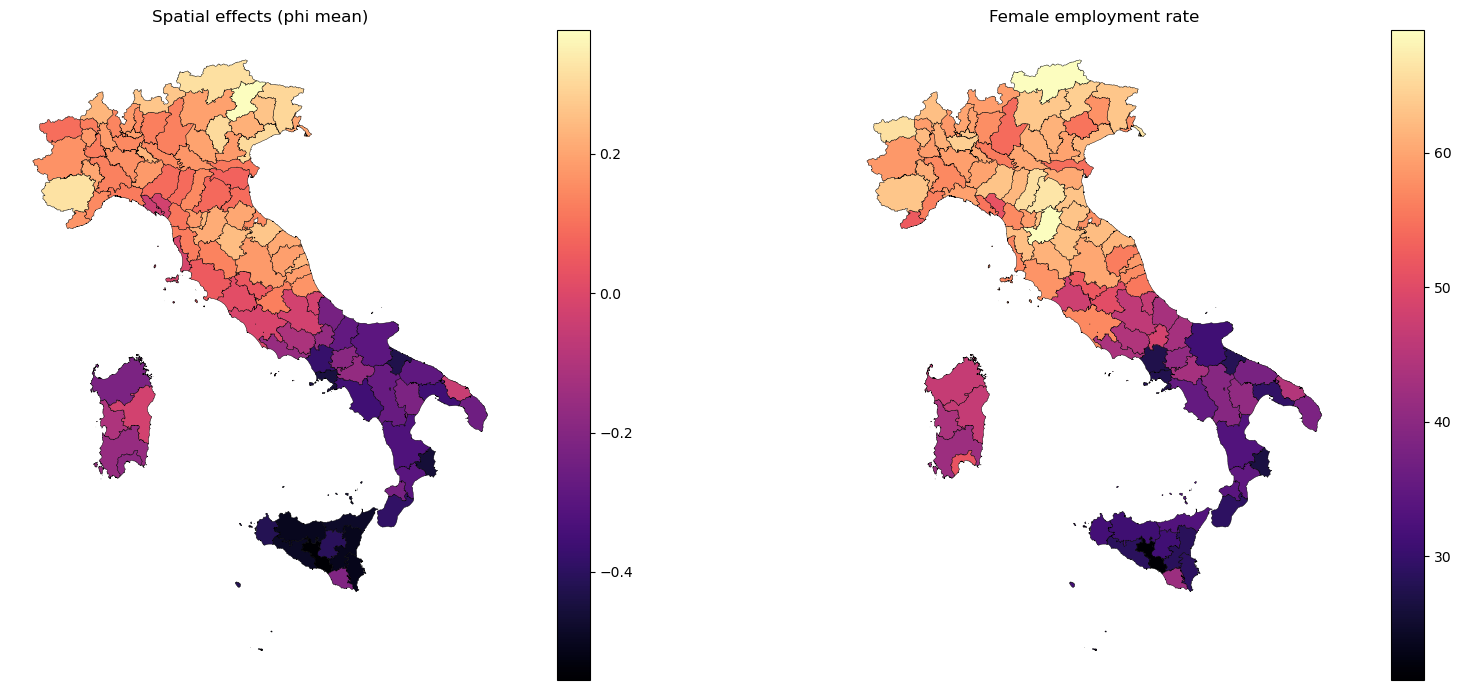
\includegraphics[width=0.7\linewidth]{pictures_second_presentation/car-vs-fem.png}
    \caption{}
    \label{fig:placeholder}
\end{figure}
\end{frame}

\begin{section}{Conclusion}

\begin{frame}{Conclusion}
\begin{itemize}
    
    \item Single cluster identified: no evidence of heterogeneous regression effects across provinces.
    
    \item High spatial correlation. 
    
    \item Public and private coverage positively affect the female employment rate.
    
    \item Possible extension: multi-year data for spatio-temporal modeling.
\end{itemize}
    
\end{frame}

\end{section}

\section{Simulation} 

\begin{frame}{Simulation Study I}

    Data generation:
    \begin{itemize}
      \item Observations: $100$ units on a $10\times 10$ grid (adjacent if sharing a boundary).
      \item Spatial effect: $\phi_i$ simulated with $\tau=1$, $\rho=0.9$.
      \item Covariates: $x_i\in\mathbb{R}^2$ i.i.d.\ Gaussian.
      \item Fixed cluster labels and cluster specific regression coefficients $\beta_k$.
      \item Outcome: $y_i=\phi_i+x_i^\top\beta_k+\varepsilon_i$, \;\; $\varepsilon_i \stackrel{\text{iid}}{\sim} \mathcal{N}(0,1)$.
      \item Experiments: $K_0=4$ and $K_0=7$.
    \end{itemize}

\end{frame}

\begin{frame}{Simulation Study II}
    \centering
    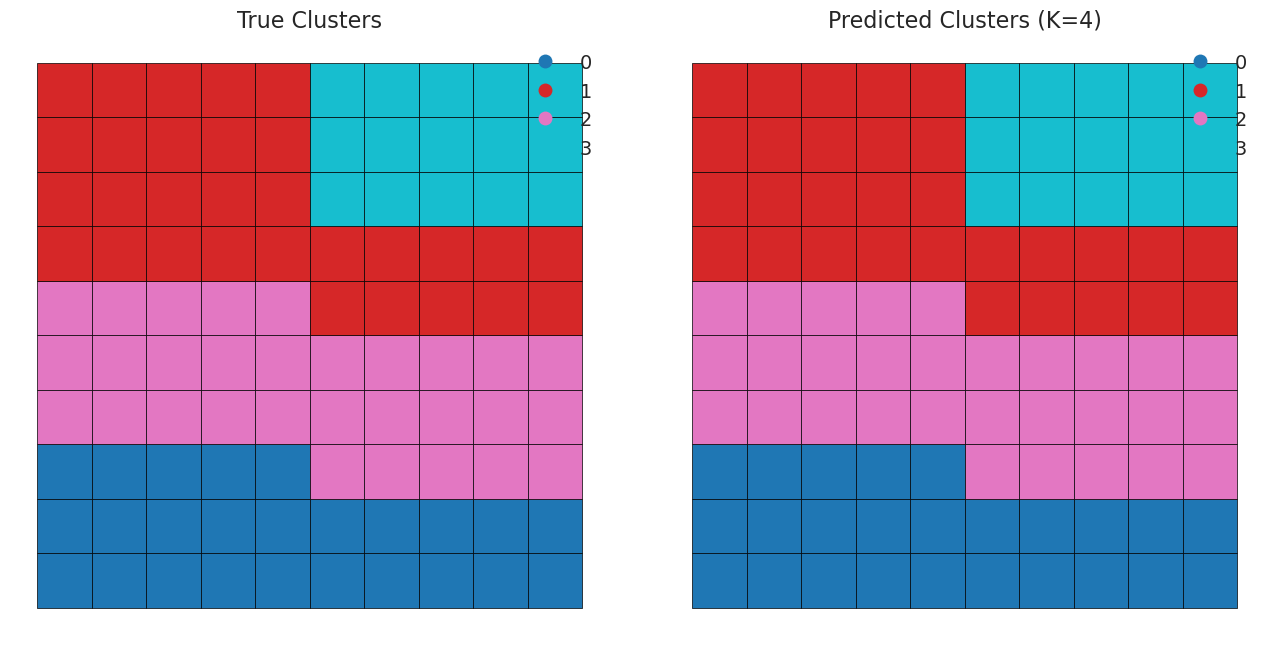
\includegraphics[width=0.7\textwidth]{pictures_second_presentation/k4-simulated.png} 

    
    \small
    Comparison between true cluster label and predicted cluster label for the model with $K_0=4$
\end{frame}

\begin{frame}{Simulation Study III}
    \centering
    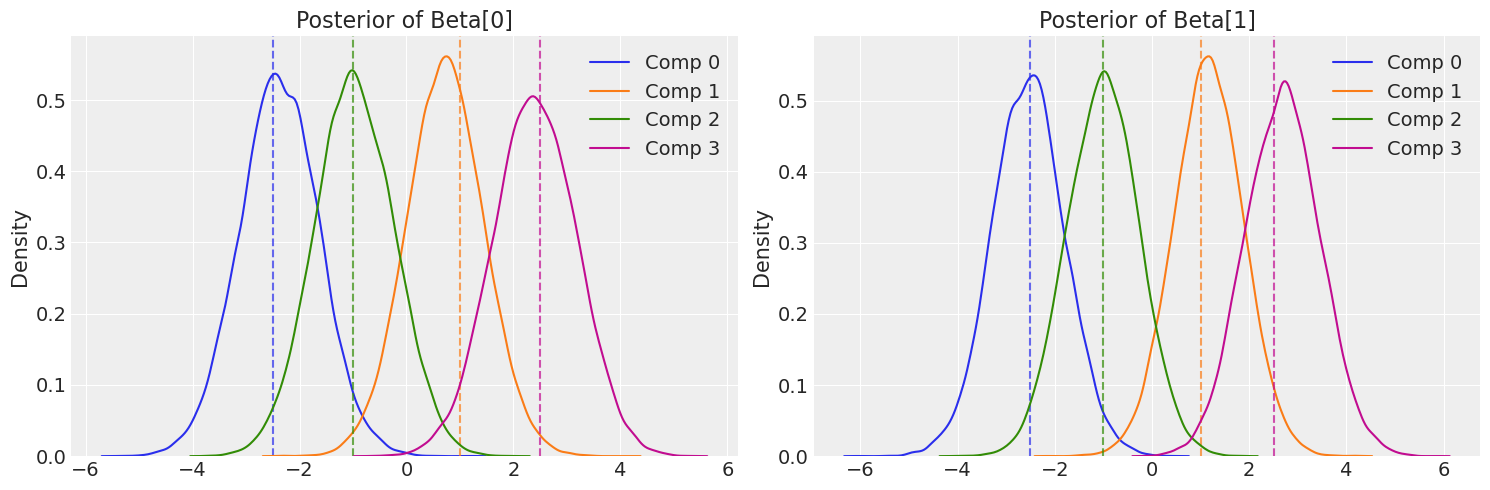
\includegraphics[width=\textwidth]{pictures_second_presentation/betaposterior-truevalue.png}

    \small
    Posterior density of the cluster-specific regression coefficients $\beta$ and their true value for the $K_0 = 4$ configuration.
\end{frame}


\begin{frame}{Simulation Study IV}
    \centering
    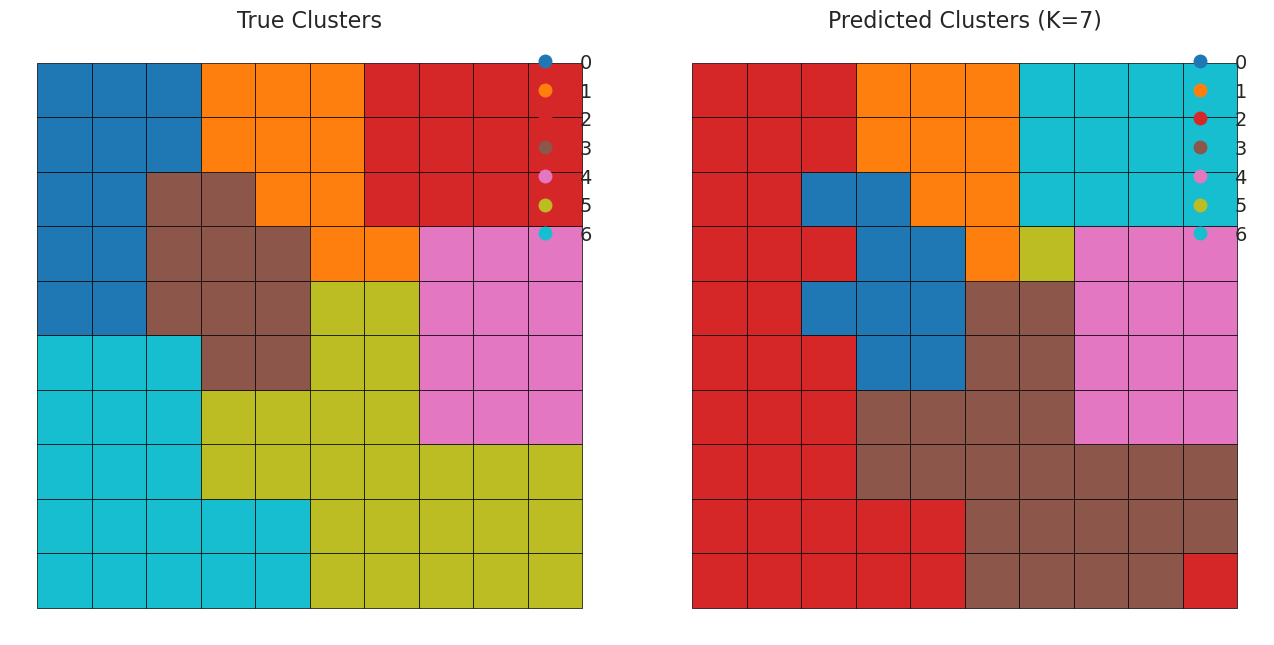
\includegraphics[width=0.7\textwidth]{pictures_second_presentation/k7-simulated.png}

    \small
    Comparison between true cluster label and predicted cluster label for the model with $K_0=7$
\end{frame}

\include{slides_second_presentation/8_Appendix}

\begin{frame}[allowframebreaks]{References}
\scriptsize
\begin{thebibliography}{99}

\bibitem[Lee(2013)]{Lee2013}
Lee, D. (2013).
\newblock CARBayes: An R Package for Bayesian Spatial Modeling with Conditional Autoregressive Priors.
\newblock \emph{Journal of Statistical Software}, 55(13), 1--24.
\newblock \url{http://doi.org/10.18637/JSS.V055.I13}

\bibitem[Park and Casella(2008)]{Park2008}
Park, T. and Casella, G. (2008).
\newblock The Bayesian Lasso.
\newblock \emph{Journal of the American Statistical Association}, 103, 681--686.
\newblock \url{http://doi.org/10.1198/016214508000000337}

\bibitem[Besag(1974)]{Besag1974}
Besag, J. (1974).
\newblock Spatial Interaction and the Statistical Analysis of Lattice Systems.
\newblock \emph{Journal of the Royal Statistical Society: Series B}, 36(2), 192--225.
\newblock \url{http://doi.org/10.1111/J.2517-6161.1974.TB00999.X}

\bibitem[Beraha et~al.(2021)]{Beraha2021}
Beraha, M., Pegoraro, M., Peli, R., and Guglielmi, A. (2021).
\newblock Spatially dependent mixture models via the logistic multivariate CAR prior.
\newblock \emph{Spatial Statistics}, 46, 100548.
\newblock \url{http://doi.org/10.1016/J.SPASTA.2021.100548}

\bibitem[Mozdzen et~al.(2022)]{Mozdzen2022}
Mozdzen, A., Cremaschi, A., Cadonna, A., Guglielmi, A., and Kastner, G. (2022).
\newblock Bayesian modeling and clustering for spatio-temporal areal data: An application to Italian unemployment.
\newblock \emph{Spatial Statistics}, 52, 100715.
\newblock \url{http://doi.org/10.1016/J.SPASTA.2022.100715}

\bibitem[Moran(1950)]{Moran1950}
Moran, P. A. P. (1950).
\newblock Notes on Continuous Stochastic Phenomena.
\newblock \emph{Biometrika}, 37(1/2), 17.
\newblock \url{http://doi.org/10.2307/2332142}

\bibitem[Anselin(1995)]{Anselin1995}
Anselin, L. (1995).
\newblock Local Indicators of Spatial Association---LISA.
\newblock \emph{Geographical Analysis}, 27(2), 93--115.
\newblock \url{http://doi.org/10.1111/J.1538-4632.1995.TB00338.X}

\bibitem[Malsiner-Walli et~al.(2014)]{Malsiner-Walli2014}
Malsiner-Walli, G., Fr\"uhwirth-Schnatter, S., and Gr\"un, B. (2014).
\newblock Model-based clustering based on sparse finite Gaussian mixtures.
\newblock \emph{Statistics and Computing}, 26(1), 303.
\newblock \url{http://doi.org/10.1007/S11222-014-9500-2}

\bibitem[Leroux et~al.(2000)]{Leroux_2000}
Leroux, B. G., Lei, X., and Breslow, N. (2000).
\newblock Estimation of Disease Rates in Small Areas: A new Mixed Model for Spatial Dependence.
\newblock In M. E. Halloran and D. Berry (eds.),
\newblock \emph{Statistical Models in Epidemiology, the Environment, and Clinical Trials}, pp. 179--191. Springer.
\newblock \url{https://doi.org/10.1007/978-1-4612-1284-3_4}

\bibitem[Binder(1978)]{Binder_1978}
Binder, D. A. (1978).
\newblock Bayesian cluster analysis.
\newblock \emph{Biometrika}, 65(1), 31--38.
\newblock \url{https://doi.org/10.1093/biomet/65.1.31}

\bibitem[Duncan et~al.(2024)]{duncan2024developing}
Duncan, E. W., Cramb, S. M., Baade, P. D., Mengersen, K. L., Saunders, T., and Aitken, J. F. (2024).
\newblock \emph{Developing a Cancer Atlas using Bayesian Methods: A Practical Guide for Application and Interpretation} (2nd ed.).
\newblock Queensland University of Technology (QUT) and Cancer Council Queensland, Brisbane.
\newblock \url{https://atlas.cancer.org.au/ebook/ebook2/Index.html}

\end{thebibliography}
\end{frame}




\end{document}

